\section{RG-Like Branch Bifurcation and Involutive Crossover in the Qubit Mean-Force Geometry}
\label{app:branch_bifurcation_involutive}

Appendix~\ref{app:branch_alignment_codex} develops the branch bookkeeping in detail.  Here we recast the same
logic in the form that is most useful for interpretation: the purity is governed by a single running scalar
$\chi$, while the apparent multiplicity resides in the continuation of the angle chart.  The resulting picture
is naturally phrased in RG-like language, but with an important caveat stated at the end of this section: for
every finite $(\beta,g)$ the exact equilibrium state is unique.

\paragraph{Running coupling, purity, and the involutive line.}
For the qubit geometry of Sec.~\ref{subsec:qubit_exact_geometry} and Sec.~\ref{sec:physical_regimes}, the exact
purity is controlled by
\begin{equation}
    \chi(\beta,g)=g^2\chi_0(\beta),
    \label{eq:branch_rg_chi_running}
\end{equation}
so that
\begin{equation}
    r(\beta,g)=\tanh\chi(\beta,g).
    \label{eq:branch_rg_purity_law}
\end{equation}
This is the sense in which $\chi$ plays the role of a running coupling (equivalently, a purity-flow variable).

The crossover $\chi=1$ defines mutually inverse maps on the monotone branch of $\chi_0(\beta)$ used throughout
the figures:
\begin{equation}
    g_\star(\beta)=\chi_0(\beta)^{-1/2},
    \qquad
    \beta_\star(g)=\chi_0^{-1}(g^{-2}),
    \label{eq:branch_rg_inverse_maps}
\end{equation}
or, equivalently,
\begin{equation}
    \chi=1
    \;\Longleftrightarrow\;
    g=g_\star(\beta)
    \;\Longleftrightarrow\;
    \beta=\beta_\star(g).
    \label{eq:branch_rg_chi1_equiv}
\end{equation}
The line $\chi=1$ is therefore self-dual (involutive) under the exchange between the two parameterizations of
the same crossover.

The formal singularity of the principal tilt-angle chart remains $\Theta=0$ (Appendix~\ref{app:branch_alignment_codex}).
What follows does not replace that statement.  Rather, it identifies $\chi=1$ as the geometrically natural
gluing locus for a branch-continuation construction that resolves the apparent reflection visible in the folded
representation of Fig.~\ref{fig:bloch_disk_portrait}.

\paragraph{A full-Bloch-circle view of the branch split.}
Figure~\ref{fig:branch_rg_bloch_bifurcation} removes the $\sqrt{m_x}$ fold and plots the same geometry in the
full coupling-plane Bloch coordinates $(m_\perp^{(\mathrm{signed})},m_z)$.  For a representative coupling
$g>g_\star^{(\mathrm{ref})}$, a single incoming branch is drawn on the high-temperature side and glued at
$T_\star(g)$ (equivalently, $\chi=1$) to the ray $\pi-\theta$.  Below $T_\star(g)$, two continuations are shown:
one returns toward the ground-state direction, while the other is the $z$-reflected continuation toward the
$\theta$ sector (equivalently, a sign-flipped branch image in the plotted transverse coordinate).  This is
exactly the bifurcation topology one wants to see in the unfolded magnetisation plane.

The key point is that the radius is never altered in this construction.  The continuation acts only on the
angular sheet, while the exact purity remains $r=\tanh\chi$.

\begin{figure*}[t]
    \centering
    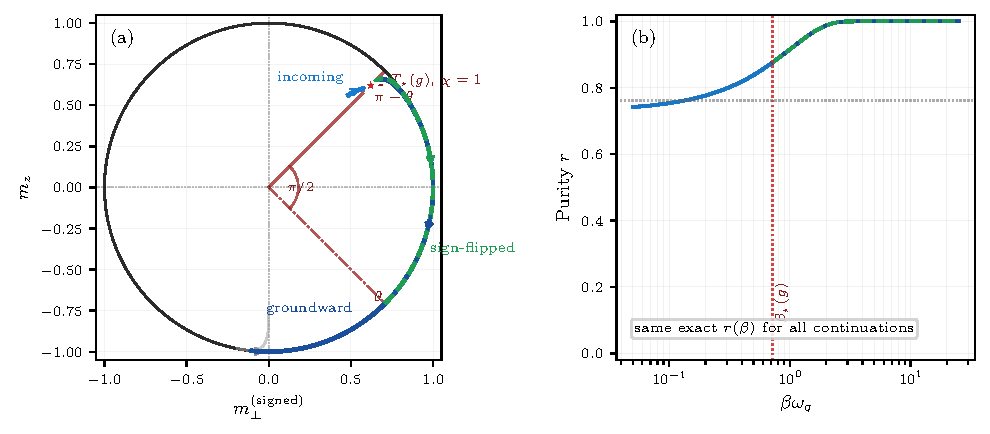
\includegraphics[width=\linewidth]{../figures/hmf_branch_bifurcation_bloch_fullcircle}
    \caption{
    Full Bloch-circle branch-continuation picture for a representative $g=1.25\,g_\star^{(\mathrm{ref})}$.
    In panel (a), the incoming branch is glued at $T_\star(g)$ (red star, $\chi=1$) to the $\pi-\theta$ ray,
    and two post-$T_\star$ continuations are shown: a ground-state-sector branch and a $z$-reflected branch
    toward the $\theta$ sector.  The pale grey curve is the exact equilibrium trajectory, included only as
    geometric context.  Panel (b) shows the corresponding purity: all displayed continuations lie on the same
    exact curve $r=\sqrt{m_z^2+m_\perp^2}=\tanh\chi$.
    }
    \label{fig:branch_rg_bloch_bifurcation}
\end{figure*}

\paragraph{The RG-like bifurcation variable.}
The relative scaling of thermal and coupling flow is captured by the single coordinate
\begin{equation}
    y\equiv \log\chi
    = \log\!\bigl(g^2\chi_0(\beta)\bigr)
    = 2\log\!\bigl(g/g_\star(\beta)\bigr),
    \label{eq:branch_rg_y_def}
\end{equation}
for which the involutive line is simply $y=0$.

In this variable the geometry becomes especially transparent: one branch sheet approaches the hub at $y=0$,
and for $y>0$ the continuation can be taken to different asymptotic angular sectors.  In the representative
construction of Fig.~\ref{fig:branch_rg_logchi_bifurcation}, the two displayed low-temperature continuations
approach the ground-state ray (on the lifted $2\pi$ sheet) and the $\theta$ sector, respectively.  The purity
panel then seals the interpretation: the apparent multiplicity is angular, not radial.

\begin{figure*}[t]
    \centering
    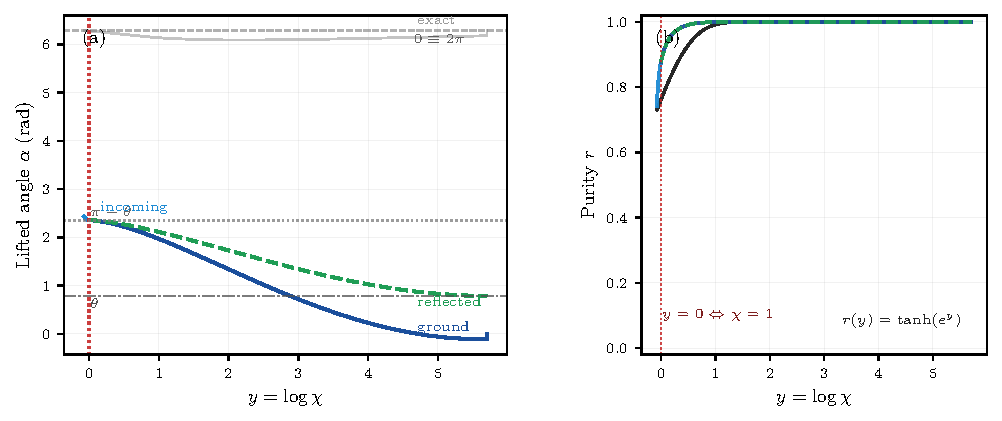
\includegraphics[width=\linewidth]{../figures/hmf_branch_bifurcation_logchi}
    \caption{
    RG-like branch bifurcation in the single flow coordinate $y=\log\chi$.  Panel (a) shows the branch sheets
    meeting at the involutive crossover $y=0$ (equivalently $\chi=1$) and separating into distinct asymptotic
    angular sectors for $y>0$.  Panel (b) shows the branch-invariant purity collapse onto the exact law
    $r(y)=\tanh(e^y)$.
    }
    \label{fig:branch_rg_logchi_bifurcation}
\end{figure*}

\paragraph{Where this lives in the \texorpdfstring{$(T,g)$}{(T,g)} plane.}
Figure~\ref{fig:branch_rg_involutive_map} plots the same structure in the parameter plane using the color field
$y=\log\chi$ and the contour $\chi=1$.  The contour is drawn both directly from $g_\star(\beta)$ and indirectly
from sampled inverse points $(\beta_\star(g),g)$; their coincidence is the numerical expression of the
involutive relation on the monotone branch of $\chi_0(\beta)$ used here.  The companion panel presents a
representative RG flow cut in the same language, comparing $\log_{10}\chi_0(\beta)$ to
$\log_{10}\chi(\beta;g_{\rm ref})$ for a fixed $g_{\rm ref}>g_\star^{(\mathrm{ref})}$, so that the crossover
appears simply as the zero crossing of the latter curve.

For the displayed domain, the sampled grid remains in the $\Theta<0$ sector, so the formal principal-chart
singularity $\Theta=0$ does not enter the plot.  This is precisely why it is useful to separate the two
statements: $\Theta=0$ is the exact singular locus of the principal tilt-angle chart, whereas $\chi=1$ is the
self-dual crossover line that organizes the continuation geometry shown here.

\begin{figure*}[t]
    \centering
    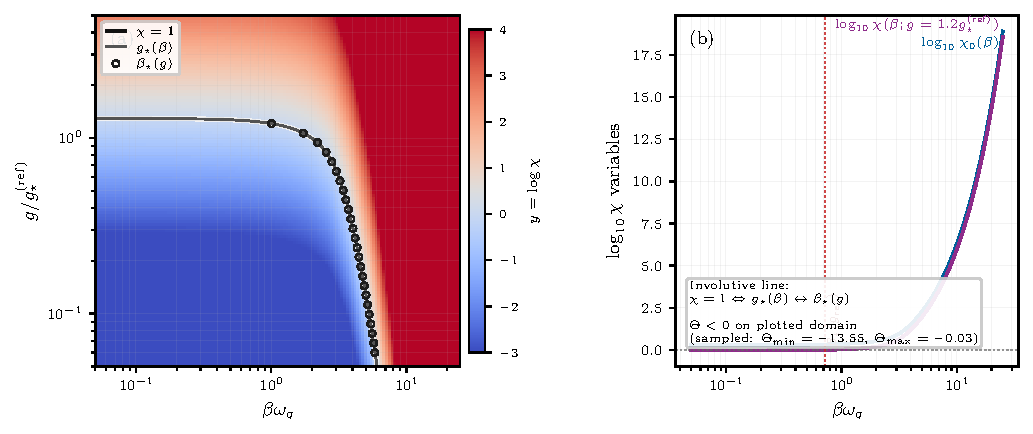
\includegraphics[width=\linewidth]{../figures/hmf_branch_bifurcation_involutive_map}
    \caption{
    Involutive crossover geometry generated by $\chi(\beta,g)=g^2\chi_0(\beta)$.  Panel (a) shows the field
    $y=\log\chi$ and the contour $\chi=1$, overlaid with both constructions of the same crossover line:
    $g_\star(\beta)$ and sampled inverse points $(\beta_\star(g),g)$.  Panel (b) shows a representative RG
    flow cut in $\log_{10}\chi$ variables: the monotone seed $\log_{10}\chi_0(\beta)$ and the driven flow
    $\log_{10}\chi(\beta;g_{\rm ref})$, with the vertical marker at $\beta_\star(g_{\rm ref})$.  The inset text
    reports the sampled $\Theta$ range, which remains negative on the plotted domain.
    }
    \label{fig:branch_rg_involutive_map}
\end{figure*}

\paragraph{Interpretation.}
The figures support an RG-like reading in which the crossover line $\chi=1$ acts as a branch-gluing threshold,
and the low-temperature continuation can be organized into distinct asymptotic angular-sector attractors (fixed
directions on the branch sheets).  The exact finite-parameter equilibrium state, however, remains single-valued.
What is multivalued here is the continuation structure of the angle chart, not the equilibrium density matrix
itself.
